\documentclass[11pt,a4paper]{article}
\usepackage[margin=2.1cm]{geometry}
\usepackage{lmodern}
\usepackage[T1]{fontenc}
\usepackage{amsmath,amssymb,bm,mathtools}
\usepackage{booktabs,array,tabularx}
\usepackage{enumitem}
\usepackage{xcolor}
\usepackage{microtype}
\setlength{\parindent}{0pt}\setlength{\parskip}{6pt plus 2pt minus 1pt}
\usepackage{caption}
\usepackage{float}
\usepackage{tikz}
\usetikzlibrary{arrows.meta,calc}
\usepackage[colorlinks=true,linkcolor=blue!55!black,urlcolor=blue!55!black,citecolor=blue!55!black]{hyperref}
\allowdisplaybreaks

% ---------- notation macros ----------
\newcommand{\vect}[1]{\bm{#1}}
\newcommand{\mat}[1]{\bm{#1}}
\newcommand{\T}{^{\mathsf{T}}}
\newcommand{\Real}{\mathbb{R}}
\newcommand{\diag}{\operatorname{diag}}
\DeclareMathOperator{\blkdiag}{blkdiag}
\newcommand{\Rot}{\mat{R}}
\newcommand{\hx}{\hat{\vect{x}}}
\newcommand{\dU}{\Delta\vect{U}}
\newcommand{\du}{\Delta\vect{u}}
\newcommand{\Ts}{T_s}
\newcommand{\Np}{N_p}
\newcommand{\Nc}{N_c}
\newcommand{\Qbar}{\bar{\mat{Q}}}
\newcommand{\Rbar}{\bar{\mat{R}}}
\newcommand{\ones}{\vect{1}}
\newcommand{\note}[1]{\par\noindent\colorbox{yellow!20}{\parbox{\dimexpr\linewidth-2\fboxsep}{\small #1}}\par}

\title{Docking State Estimator and MPC for a Mecanum Barrier Robot\\[4pt]
\large Design formulation, first pass}
\author{Working document for the P4P thesis}
\date{8 October 2026}

\begin{document}
\maketitle

\begin{abstract}
\noindent This document writes out the estimator and controller formulation for the docking manoeuvre, for both the full-scale theoretical system and the tabletop demonstrator. The structure follows the MECHENG~724 notes: the predictor--corrector Kalman filter of Section~4 is extended to a multi-rate EKF with a delayed correction, and the augmented incremental MPC of Section~5 is extended to a successively linearised MPC with docking-specific constraints. Section~\ref{sec:decisions} answers the open design questions (frame choice, inverse kinematics inside or outside the MPC, kinematic versus lag model) with the trade-offs written out.
\end{abstract}

\tableofcontents

% =====================================================================
\section{Frames, geometry and notation}
\label{sec:frames}

\begin{figure}[H]
\centering
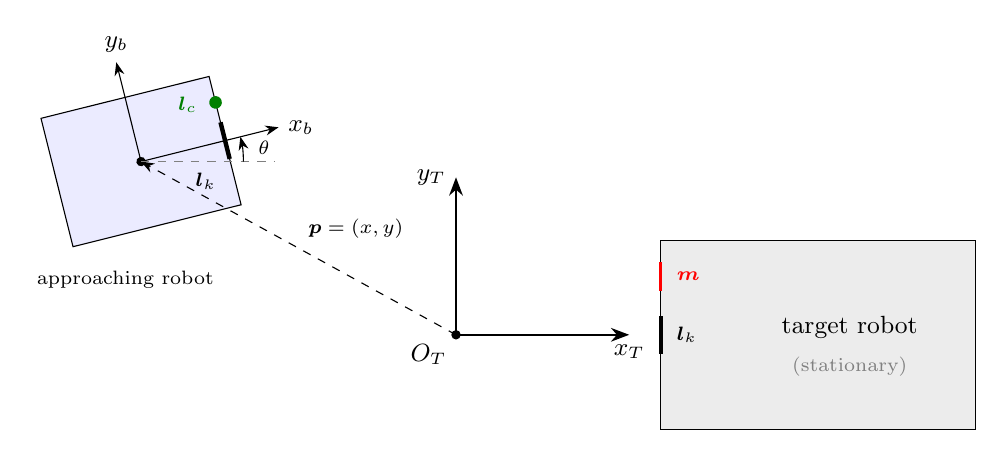
\begin{tikzpicture}[scale=2.0,>=Stealth,font=\small]
  % target frame axes
  \draw[->,thick] (0,0) -- (1.1,0) node[below] {$x_T$};
  \draw[->,thick] (0,0) -- (0,1.0) node[left] {$y_T$};
  \fill (0,0) circle (0.03) node[below left] {$O_T$};
  % target robot (stationary)
  \draw[fill=gray!15] (1.3,-0.6) rectangle (3.3,0.6);
  \node at (2.5,0.05) {target robot};
  \node[font=\scriptsize,gray] at (2.5,-0.2) {(stationary)};
  \draw[ultra thick] (1.3,-0.12) -- (1.3,0.12);
  \node[font=\scriptsize,anchor=west] at (1.34,0) {$\vect l_k$};
  \draw[very thick,red] (1.3,0.28) -- (1.3,0.46);
  \node[font=\scriptsize,red,anchor=west] at (1.34,0.37) {$\vect m$};
  % approaching robot
  \begin{scope}[shift={(-2.0,1.1)},rotate=14]
    \draw[fill=blue!8] (-0.55,-0.42) rectangle (0.55,0.42);
    \draw[->] (0,0) -- (0.9,0) node[right] {$x_b$};
    \draw[->] (0,0) -- (0,0.65) node[above] {$y_b$};
    \fill (0,0) circle (0.03);
    \fill[green!50!black] (0.55,0.25) circle (0.04);
    \node[font=\scriptsize,green!50!black,anchor=east] at (0.49,0.25) {$\vect l_c$};
    \draw[ultra thick] (0.55,-0.12) -- (0.55,0.12);
    \node[font=\scriptsize,anchor=east] at (0.49,-0.25) {$\vect l_k$};
  \end{scope}
  \node[font=\scriptsize] at (-2.1,0.35) {approaching robot};
  % position vector and heading
  \draw[->,dashed] (0,0) -- (-2.0,1.1) node[pos=0.5,above right,font=\scriptsize] {$\vect p=(x,y)$};
  \draw[dashed,gray] (-2.0,1.1) -- (-1.15,1.1);
  \draw[->] (-1.35,1.1) arc (0:14:0.65);
  \node[font=\scriptsize] at (-1.22,1.19) {$\theta$};
\end{tikzpicture}
\caption{Target frame $T$ and body frame $b$. Thick ticks are the two halves of the genderless coupler, the green dot is the camera at $\vect l_c$ in the body frame, the red tick is the fiducial marker. The origin $O_T$ is where the chassis centre of the approaching robot sits when the couplers are mated, so the docked reference pose is $(0,0,0)$ and the approach comes from $x<0$. The target's coupler is therefore at $\vect{l}_k$ in $T$ and the marker at $\vect{m}=\vect{l}_k+\vect{d}_{mk}$, where $\vect{d}_{mk}$ is the known coupler-to-marker offset.}
\label{fig:frames}
\end{figure}

\paragraph{Frames.}
\begin{itemize}[nosep]
  \item $T$: target frame, fixed to the stationary target robot. Since the target is parked, $T$ is an inertial frame. Everything the docking controller cares about is expressed here.
  \item $b$: body frame of the approaching robot, origin at the chassis kinematic centre, $x_b$ forward.
  \item $W$: world frame (RTK-GPS, full scale only). Used by the navigation filter and at handover; the docking filter never sees it.
\end{itemize}

\paragraph{Symbols.}
\begin{align}
\Rot(\theta) &= \begin{bmatrix}\cos\theta & -\sin\theta\\ \sin\theta & \cos\theta\end{bmatrix}, &
\vect{p} &= \begin{bmatrix} x \\ y \end{bmatrix} \ \text{(chassis centre in $T$)}, &
\theta &= \text{heading of } x_b \text{ relative to } x_T, \\
\vect{v} &= \dot{\vect{p}} \ \text{(velocity in $T$)}, &
\vect{v}_b &= \Rot(\theta)\T \vect{v} = \begin{bmatrix} u_b \\ v_b\end{bmatrix} \ \text{(velocity in $b$)}, &
r &= \dot\theta \ \text{(yaw rate)}.
\end{align}
Constant geometry: $\vect{l}_c$ camera position in $b$, $\vect{l}_k$ coupler position in $b$ (and, by construction of $T$, the target coupler position in $T$), $\vect{m}$ marker position in $T$. The robot's coupler position in $T$ is $\vect{p}+\Rot(\theta)\vect{l}_k$, which equals $\vect{l}_k$ exactly when $(x,y,\theta)=(0,0,0)$.

\paragraph{Sampling.} IMU at $f_{\mathrm{imu}}=200$~Hz ($T=5$~ms), fiducial pose solver at 15~Hz with a known capture-to-availability delay $\tau_d=50$~ms, RTK-GPS at 10~Hz (full scale only), MPC at $1/\Ts = 20$~Hz.

% =====================================================================
\section{Design decisions and the alternatives considered}
\label{sec:decisions}

\subsection{Docking tolerances and what the controller actually targets}
\label{sec:tol}

The genderless coupler defines the pass/fail band. Of its six degrees of freedom only three are controllable by a planar chassis: longitudinal $x$, lateral $y$ and yaw $\theta$. Vertical offset and pitch are set by the deck surface and the suspension; they are \emph{monitored} from the 6-DOF pose solution (as an abort criterion) but not controlled.

\begin{table}[H]
\centering
\begin{tabular}{lcccc}
\toprule
 & horizontal & vertical & yaw & pitch \\
\midrule
Demonstrator coupler tolerance & $\pm 12$~mm & $\pm 6$~mm & $\pm 20^\circ$ & $\pm 10^\circ$ \\
Full-scale coupler tolerance   & $\pm 80$~mm & $\pm 40$~mm & $\pm 20^\circ$ & $\pm 10^\circ$ \\
Controlled by the planar controller? & yes & no & yes & no \\
\bottomrule
\end{tabular}
\caption{Coupler capture tolerances. Horizontal means lateral at the coupler, i.e. the $y$ error of the coupler point, not of the chassis centre.}
\end{table}

Two consequences for the design:
\begin{enumerate}[nosep]
  \item \textbf{Internal targets are tighter than the tolerance.} The controller aims for zero, but the weights are set so that the closed loop is driven well inside the band, leaving margin for estimation error and the coupler's capture cone. A working rule is one third of the tolerance: $y_{\mathrm{tgt}} = 4$~mm (demo), $27$~mm (full scale).
  \item \textbf{Yaw matters through the lever arm.} The lateral error at the coupler is $y + L_k\sin\theta$, where $L_k$ is the longitudinal distance from the chassis centre to the coupler. A yaw error of $\theta$ therefore costs $L_k\theta$ of lateral tolerance, so the useful yaw target is
  \begin{equation}
    \theta_{\mathrm{tgt}} \approx \frac{y_{\mathrm{tgt}}}{L_k}
    \qquad\Rightarrow\qquad
    \theta_{\mathrm{tgt}} \approx 1.5^\circ \ \text{for } L_k=0.15\text{ m (demo) or } L_k = 1\text{ m (full scale)},
  \end{equation}
  far tighter than the $\pm 20^\circ$ of the coupler itself. The heading target feeds Bryson's rule for the MPC weights in Section~\ref{sec:cost}; the position weights use the tolerance itself, for a reason given there, and the targets remain the pass criteria of the closed-loop tests.
\end{enumerate}

\subsection{Which frame to estimate in (question 9)}
\label{sec:frame}

Four formulations were considered. In all of them the IMU inputs are body-frame quantities and the fiducial measures the relative pose, so the difference is only \emph{where the nonlinearity sits} and how awkward the bookkeeping is.

\begin{table}[H]
\centering
\small
\renewcommand{\arraystretch}{1.25}
\begin{tabularx}{\linewidth}{>{\raggedright\arraybackslash}p{2.7cm} X X}
\toprule
Option & Pros & Cons \\
\midrule
\textbf{A. Target frame, velocity in $T$} \newline
$\vect{x}=[x,y,\theta,v_x,v_y]$ \newline
\emph{(recommended)} &
Position rows are linear ($\dot{\vect p}=\vect v$). Only nonlinearity is rotating the accelerometer by $\theta$. No Coriolis terms. Fiducial measurement is linear, $\mat H=[\mat I\ \mat 0]$. Reference is the constant $(0,0,0)$. MPC uses $\vect v$ directly as $\Delta\vect{x}/\Ts$. Identical for theory and demo. &
Handover from a world-frame navigation filter needs one rotation of the state and covariance (cheap, done once). Body-frame velocity, if wanted, is a derived quantity $\Rot\T\vect v$. \\
\midrule
\textbf{B. Target frame, velocity in $b$} \newline
$\vect{x}=[x,y,\theta,u_b,v_b]$ &
Velocity states match what the wheel kinematics produce, so a wheel-speed measurement model would be linear. Accelerometer enters without rotation. &
Velocity rows gain the rotating-frame terms $\dot u_b = a_x + r v_b$, $\dot v_b = a_y - r u_b$ (bilinear). Position rows become nonlinear ($\dot{\vect p}=\Rot(\theta)\vect v_b$). Mathematically equivalent to A (a state transformation), just a worse place to put the nonlinearity. \\
\midrule
\textbf{C. Body frame, target pose as the state} \newline
$\vect{x}=[\vect{p}_t^{\,b},\theta_t,\ldots]$ \newline
\emph{(original idea)} &
Fiducial measurement is directly in the camera/body frame. IMU inputs need no rotation. &
The frame itself rotates, so the target position obeys $\dot{\vect p}_t^{\,b} = -\vect v_b - r\,\mat S\vect p_t^{\,b}$ with $\mat S$ the $90^\circ$ rotation: every row is bilinear in state and input. Any world information (GPS fix, target pose from fleet comms) must be rotated into a moving frame, so those measurement models become state dependent. Covariance at handover must be transformed through the current heading. Linearisation point for the MPC changes with every rotation. More algebra for no accuracy gain. \\
\midrule
\textbf{D. World frame, robot + target poses} \newline
$\vect{x}=[\vect{p}_r,\theta_r,\vect v_r,\vect{p}_t,\theta_t]$ (8 states) &
One filter for navigation and docking; GPS stays in the loop; the target's world pose is refined by the fiducial. &
Fiducial model $h=\Rot(\theta_t)\T(\vect p_r-\vect p_t)$ is nonlinear in both poses. Without GPS (the demo) the robot and target poses are only observable through their difference, so the filter reduces to option A anyway. The MPC needs the \emph{relative} pose, a derived quantity whose covariance has to be propagated. Three more states, more Jacobians, and the dynamic-allocation problem you identified. \\
\bottomrule
\end{tabularx}
\caption{Frame options for the docking estimator.}
\end{table}

\noindent\textbf{Decision: option A (locked, 8 October 2026).} Its one real cost, the handover transformation, is a single rotation
\begin{gather}
\hx_0 = \begin{bmatrix}\Rot(\theta_t)\T(\hat{\vect p}_W-\vect p_{t,W}) \\ \hat\theta_W-\theta_t \\ \Rot(\theta_t)\T\hat{\vect v}_W\end{bmatrix},
\qquad
\mat T=\blkdiag\!\big(\Rot(\theta_t)\T,\ 1,\ \Rot(\theta_t)\T\big),
\label{eq:handover}\\
\mat P_0 = \mat T\,\mat P_W\,\mat T\T + \blkdiag(\mat P_{\mathrm{tgt}},\ \mat 0),
\end{gather}
executed once when the fleet allocates the target. Dynamic allocation is then just instantiating the docking filter with that target's $(\vect p_{t,W},\theta_t,\vect m)$; the state never grows.

For the full-scale system the unified-filter benefit of option D is real: no mode switch, and continuity of a world-frame estimate through a marker dropout. The first is recovered in A by (\ref{eq:handover}). The second is deliberately not pursued: a world-frame fix mapped into the target frame is only as good as the target's reported pose, a few centimetres, so the docking filter coasts on the IMU through short dropouts and the supervisor reverts to navigation after a timeout (Section~\ref{sec:gpsrole}). The relative-pose accuracy is the same in A and D, because only the fiducial carries relative information and GPS error is common to robot and target, so it cancels in the difference provided the cross-covariance is tracked. If world-frame consistency during docking is ever required, the right form is A plus three target-pose states, not the world parameterisation: the precision sensor then stays linear and the coarse sensor carries the nonlinearity.

The parallel to the navigation filter is also tighter in A than in D. Navigation at full scale is the same five-state filter written in $W$: identical process model and Jacobians, with the RTK position and the INS heading as linear measurements in place of the fiducial (Table~\ref{tab:template}). Under D the docking filter would have eight states and the navigation filter five, and carrying the three target states permanently would leave them unobservable whenever no target is allocated.

\begin{table}[H]
\centering
\small
\renewcommand{\arraystretch}{1.2}
\setlength{\tabcolsep}{4pt}
\begin{tabular}{lll}
\toprule
 & Navigation (full scale, theory) & Docking (full scale and demo) \\
\midrule
Frame & world $W$ & target $T$ \\
State & $[x,y,\theta,v_x,v_y]$ in $W$ & $[x,y,\theta,v_x,v_y]$ in $T$ \\
Inputs & $a_x,a_y,r$ from the IMU & same \\
Process model, Jacobians & (\ref{eq:f}), (\ref{eq:FG}) & same \\
Measurements & RTK position + INS heading, $\mat H=[\mat I_3\ \mat 0]$ & fiducial pose, $\mat H=[\mat I_3\ \mat 0]$, gated \\
 & & marker loss: supervisor \\
Transition & \multicolumn{2}{l}{one rotation of state and covariance, (\ref{eq:handover}), when the marker is acquired} \\
MPC reference & lane path, time-varying, long horizon & docked pose, constant, short horizon \\
\bottomrule
\end{tabular}
\caption{One five-state estimator template instantiated twice. Only the frame label, the measurement rows and the MPC reference differ.}
\label{tab:template}
\end{table}

\subsection{Inverse kinematics: inside or outside the MPC (question 6)}
\label{sec:ik}

There are three distinct ways the inverse kinematics $\mat J^{-}$ (Appendix~\ref{app:mecanum}) can ``be in'' the MPC:

\begin{enumerate}[nosep]
  \item \textbf{As decision variables.} Let the four wheel speeds $\vect\omega\in\Real^4$ be the inputs. The pose prediction only depends on $\mat J^{+}\vect\omega$ (the forward kinematics), which has a one-dimensional null space $\vect n=[1,1,-1,-1]\T$: front wheels forward, rear wheels backward, pure scrubbing. A kinematic model predicts \emph{zero} pose change for that combination, so the Hessian is singular along $\vect n$ unless $\Rbar$ regularises it, in which case the optimiser simply sets that component to zero. You pay a fourth decision variable per step and get nothing back, because the model cannot predict what slip does.
  \item \textbf{As constraints.} Keep the three body velocities $\vect u=[u_b,v_b,r_b]\T$ as decision variables and impose the per-wheel speed limits through $\mat J^{-}$: $-\omega_{\max}\ones \le \mat J^{-}\vect u \le \omega_{\max}\ones$. This is exact, linear in the decision variables, and is what makes the controller respect the motors. \textbf{This is the recommended form}, and it is what ``including the inverse kinematics in the MPC'' should mean here.
  \item \textbf{As the actuator model.} If the wheel-speed loops are slow enough to matter, their lag belongs in the prediction model. That is question~7.
\end{enumerate}

\subsection{Kinematic model versus first-order lag, and how it interacts with question 6 (question 7)}
\label{sec:lag}

With body velocities as the decision variables, the plant seen by the MPC is ``command $\to$ wheel PID $\to$ actual body velocity $\to$ pose''. The two candidate models differ in whether the middle step is instantaneous.

\textbf{Pure kinematic (baseline).} Actual velocity equals the command: $\vect v_b = \vect u$. States are the pose only. This is your stated assumption and the course's setting. The incremental $\du$ formulation still gives smooth commands because increments are penalised and bounded, so acceleration limits are respected even though the model has no inertia.

\textbf{First-order lag (refinement).} Each wheel loop is modelled as $\dot\omega_i = (\omega_{i,\mathrm{cmd}}-\omega_i)/\tau$. Because $\mat J^{-}$ and $\mat J^{+}$ are constant linear maps and all four motors share the same $\tau$, the lag commutes with the kinematics:
\begin{equation}
\dot{\vect\omega} = \tfrac{1}{\tau}(\vect\omega_{\mathrm{cmd}}-\vect\omega)
\;\Rightarrow\;
\dot{\vect v}_b = \mat J^{+}\dot{\vect\omega} = \tfrac{1}{\tau}\big(\mat J^{+}\mat J^{-}\vect u - \mat J^{+}\vect\omega\big) = \tfrac{1}{\tau}(\vect u-\vect v_b),
\end{equation}
using $\mat J^{+}\mat J^{-}=\mat I_3$. So a per-axis lag on the body velocity is \emph{exact} for identical motors, which is why question 7 does not force wheel speeds to be decision variables. The lag model adds three velocity states to the MPC model (Section~\ref{sec:lagmodel}); the EKF already estimates them.

\textbf{Decision.} Start with the kinematic model. Identify $\tau$ from a step test on the demonstrator; adopt the lag model if $\tau$ is comparable to $\Ts$ or larger (on a 600~kg chassis it almost certainly is, so the full-scale model should carry it). The closed-loop harness shows the cost of ignoring the lag directly: the kinematic MPC stops the \emph{command} at the contact plane, and the chassis then overshoots by about $v_{\mathrm{final}}\,\tau$, 15~mm at full scale with $\tau = 0.3$~s and 5~mm on the demonstrator with $\tau = 0.1$~s. The lag model predicts the coast and removes it.

\subsection{Role of RTK-GPS during docking}
\label{sec:gpsrole}

None inside the docking loop. RTK brings the robot into marker range in navigation mode and can seed the handover (\ref{eq:handover}); once the marker is acquired, the docking filter runs on the IMU and the fiducial alone. The reasons are quantitative. Relative accuracy between two independent RTK fixes is roughly $\sqrt{2}\times 20$~mm $\approx 28$~mm ($1\sigma$), plus the uncertainty of the target's reported pose, so a world-frame fix mapped into the target frame is good to a few centimetres: useless against the demonstrator's $\pm 12$~mm and marginal against the full-scale $\pm 80$~mm, while the fiducial is better by an order of magnitude whenever it is visible. During a short marker dropout the IMU coast is already comparable: in the harness a 2~s outage costs about 55~mm at the full-scale noise levels, against about 30~mm with an RTK fallback. Keeping RTK out of the docking loop removes a dependency on the target's reported pose, removes the covariance bookkeeping that a constant target-pose error would require, and makes the theory and demonstrator docking filters identical rather than merely alike. Marker loss is therefore a supervisor matter: hold position, and after a timeout revert to navigation mode, where RTK position and INS heading are the measurements (Table~\ref{tab:template}). The coast-duration experiment of Section~\ref{sec:verif} sets that timeout.

\subsection{Compute and deployment}
The demonstrator runs ROS nodes on a Raspberry Pi~5. A 5-state EKF at 200~Hz and a 30-variable QP at 20~Hz are both comfortably within budget in Python with NumPy and OSQP. Design and proof are done in MATLAB/Simulink with \texttt{quadprog}; the deployed nodes are a port of the same equations, with the Simulink model as the reference for regression tests.

\subsection{IMU grade: demonstrator versus full scale}
\label{sec:imu}
The demonstrator uses a Bosch BNO085, a consumer MEMS part with onboard fusion. Its magnetometer-fused heading is unreliable near motors and would be useless on a steel bridge, so on the demonstrator only the gyro yaw rate is used as a filter input (the ``game rotation vector'' path, which excludes the magnetometer) and the fiducial fixes the heading. The full-scale robot will carry a higher-grade unit, most likely an industrial MEMS GNSS/INS with dual-antenna RTK heading, which also absorbs the separate RTK receiver and gives the navigation mode a direct heading measurement. The estimator structure of Section~\ref{sec:ekf} does not change with that choice; only the input noise $\mat\Sigma_u$, the validity of the no-bias-state assumption, and an optional heading measurement row differ. The selection study for the full-scale unit is a separate document, \texttt{design/imu\_options\_fullscale.md}.

Its conclusions, in brief. In-run bias instability is not the limiting parameter for any grade of sensor; what decides whether the no-bias-state model holds is the \emph{residual} yaw-gyro bias left after the unit's own estimator, and the accelerometer channel is dominated by gravity leakage from attitude error rather than by accelerometer bias ($0.05^\circ$ of tilt error is $0.9$~mg). The recommended unit is a dual-antenna RTK GNSS/INS such as the HBK/MicroStrain 3DM-GQ7 or the SBG Ellipse-D: $0.05^\circ$ roll and pitch for gravity compensation, a direct heading measurement at $0.2$ to $0.25^\circ$, built-in RTK, IP68 and official ROS~2 drivers, at roughly US\$4000 per unit. The fleet-cost alternative is an industrial MEMS module (Xsens MTi-7/8 class) with two u-blox ZED-F9P receivers in moving-base mode, or a Septentrio mosaic-H, at US\$600 to 1300 in parts. The parameter sheet carries GQ7-class noise values for the full-scale model.

% =====================================================================
\section{State estimator}
\label{sec:ekf}

\subsection{State, inputs and continuous model}
\begin{equation}
\vect x = \begin{bmatrix} x \\ y \\ \theta \\ v_x \\ v_y \end{bmatrix}\in\Real^5,
\qquad
\vect u_{\mathrm{imu}} = \begin{bmatrix} a_x \\ a_y \\ r \end{bmatrix}
\ \text{(gravity-compensated body-frame acceleration, gyro yaw rate)}.
\end{equation}
\begin{equation}
\dot x = v_x,\qquad \dot y = v_y,\qquad \dot\theta = r,\qquad
\begin{bmatrix}\dot v_x\\ \dot v_y\end{bmatrix} = \Rot(\theta)\begin{bmatrix}a_x\\ a_y\end{bmatrix}
=\begin{bmatrix}\cos\theta\,a_x-\sin\theta\,a_y\\ \sin\theta\,a_x+\cos\theta\,a_y\end{bmatrix}.
\label{eq:ct}
\end{equation}
No motion model, no wheel model, no slip states: the IMU reports what the chassis actually does. The yaw rate is an input rather than a state, for the same reason acceleration is: the IMU measures it directly, it has no dynamics we model, and no other sensor observes it. Velocity earns its place as a state because the position fixes constrain how fast position changes, so the filter has a second source of information to fuse with the accelerometer. Yaw rate has no such second source; a rate obtained by differencing the 15~Hz fiducial heading would have a noise of order $10^\circ$/s against the gyro's $0.03^\circ$/s. A yaw-rate state would therefore need an invented random-walk process model, would be driven only by the gyro and corrected by nothing, and would return a slightly smoothed gyro reading that the heading integration does not benefit from. The one related state that could be justified is a gyro \emph{bias}, observable through the fiducial heading over time; Section~\ref{sec:imu} shows the full-scale unit does not need it, and the demonstrator covers its larger residual through $\mat Q_{\mathrm{floor}}$ instead. The MPC's initial increment uses the yaw rate straight from the gyro.

\subsection{Discrete prediction and Jacobians}
Euler integration at the IMU period $T$ is adequate at 200~Hz:
\begin{equation}
\vect x_{k+1} = \vect f(\vect x_k,\vect u_k) =
\begin{bmatrix}
x + T v_x \\
y + T v_y \\
\theta + T r \\
v_x + T(\cos\theta\,a_x - \sin\theta\,a_y) \\
v_y + T(\sin\theta\,a_x + \cos\theta\,a_y)
\end{bmatrix}.
\label{eq:f}
\end{equation}
\begin{gather}
\mat F_k = \left.\frac{\partial\vect f}{\partial\vect x}\right|_{\hx_{k},\vect u_k} =
\begin{bmatrix}
1 & 0 & 0 & T & 0 \\
0 & 1 & 0 & 0 & T \\
0 & 0 & 1 & 0 & 0 \\
0 & 0 & -T(\sin\theta\,a_x+\cos\theta\,a_y) & 1 & 0 \\
0 & 0 & \phantom{-}T(\cos\theta\,a_x-\sin\theta\,a_y) & 0 & 1
\end{bmatrix},
\label{eq:FG}\\
\mat G_k = \frac{\partial\vect f}{\partial\vect u_{\mathrm{imu}}} =
\begin{bmatrix}
0 & 0 & 0 \\
0 & 0 & 0 \\
0 & 0 & T \\
T\cos\theta & -T\sin\theta & 0 \\
T\sin\theta & \phantom{-}T\cos\theta & 0
\end{bmatrix}.
\end{gather}
Process noise enters through the IMU inputs, so
\begin{equation}
\mat Q_k = \mat G_k\,\mat\Sigma_u\,\mat G_k\T + \mat Q_{\mathrm{floor}},
\qquad
\mat\Sigma_u = \diag(\sigma_a^2,\sigma_a^2,\sigma_r^2),
\label{eq:Q}
\end{equation}
with $\sigma_a,\sigma_r$ the per-sample noise standard deviations (from the datasheet noise density, or measured on the bench) and $\mat Q_{\mathrm{floor}}$ a small diagonal for conditioning. Residual accelerometer bias and any gravity leak from an imperfect onboard attitude are not modelled as states; they are absorbed by inflating the velocity entries of $\mat Q$, exactly the ``treat $Q$ as a tuning parameter'' guidance of the course notes. In the implementation the velocity and heading entries of $\mat Q_{\mathrm{floor}}$, $q_v$ and $q_\theta$, are tuning parameters chosen the way the notes prescribe: swept over a decade either side and set where the filter is consistent, i.e.\ where the 20-run NEES of Section~3.8 sits near its ideal value with the marker visible. Too small and the filter trusts its IMU integration over the fixes, becoming sluggish and overconfident whenever something the IMU cannot see occurs; too large and it re-derives velocity from every fix and becomes noisy. A useful interpretation when reading the chosen values: a per-step variance $q$ produces $\sqrt{q\,t/T}$ of uncertainty after $t$ seconds, so the full-scale $q_v$ corresponds to tolerating a residual input bias of $0.01$~m/s$^2$ over $3$~s.

\paragraph{Predictor step} (every IMU sample):
\begin{equation}
\hx_{k|k-1} = \vect f(\hx_{k-1|k-1},\vect u_k),\qquad
\mat P_{k|k-1} = \mat F_k\mat P_{k-1|k-1}\mat F_k\T + \mat Q_k.
\end{equation}

\subsection{Fiducial measurement}
\label{sec:fid}
The pose solver returns the marker's 6-DOF pose in the camera frame. Take its planar translation $\vect t\in\Real^2$ and yaw $\psi$. With the marker frame aligned with $T$ and the camera aligned with $x_b$ at $\vect l_c$,
\begin{equation}
\theta_z = \psi_0 - \psi,
\qquad
\vect p_z = \vect m - \Rot(\theta_z)\,(\vect t + \vect l_c),
\end{equation}
where $\psi_0$ is a constant mounting offset. The remaining components (height, pitch, roll) are logged for the tolerance check of Section~\ref{sec:tol}. The pseudo-measurement is linear in the state:
\begin{equation}
\vect z = \begin{bmatrix}\vect p_z\\ \theta_z\end{bmatrix} = \mat H\vect x + \vect v,
\qquad
\mat H = \begin{bmatrix}\mat I_3 & \mat 0_{3\times 2}\end{bmatrix},
\qquad
\mat R_f = \diag(\sigma_p^2,\sigma_p^2,\sigma_\theta^2).
\label{eq:Hf}
\end{equation}
$\mat R_f$ is measured on the bench with the robot static at a few ranges; if it grows noticeably with range, use $\mat R_f(d)=\mat R_{f,0}\,(1+(d/d_0)^2)$. The growth has a geometric cause: the transform above rotates the camera-to-marker vector by the measured yaw, so a yaw error $\delta\psi$ shifts the derived position by about $|\vect t+\vect l_c|\,\delta\psi$, which is $9$~mm for $0.5^\circ$ at $1$~m. Strictly this makes $\mat R_f$ non-diagonal; propagating the solver's covariance through the transform is a refinement, and the range-scaled diagonal is adequate at docking ranges. This is the only place in the design where yaw accuracy couples into position; the state propagation itself does not depend on it, because the target frame is inertial and the chassis centre does not move when the robot rotates.

\paragraph{Corrector step} (every fiducial arrival):
\begin{gather}
\vect\nu = \vect z - \mat H\,\hx(t_c),\qquad
\mat S = \mat H\mat P\mat H\T + \mat R_f,\qquad
\mat K = \mat P\mat H\T\mat S^{-1},
\label{eq:corr}\\
\hx \leftarrow \hx + \mat K\vect\nu,\qquad
\mat P \leftarrow (\mat I-\mat K\mat H)\mat P.
\end{gather}
This is the course's corrector written with the innovation named explicitly; $\mat P-\mat K\mat C\mat P$ in the notes is the same update.

\subsection{Delay compensation}
\label{sec:delay}
The measurement available at $t_k$ was captured at $t_c = t_k-\tau_d$. The filter keeps a ring buffer of $(t,\hx)$ at the IMU rate (10 entries cover 50~ms). The innovation in (\ref{eq:corr}) is formed against the \emph{buffered} estimate $\hx(t_c)$, and the correction $\mat K\vect\nu$ is applied to the \emph{present} estimate. The exact treatment (Larsen's method) would scale $\mat K$ by the state transition from $t_c$ to $t_k$; over 50~ms at docking speeds that transition is within a few per cent of the identity, so the simple form is used. The uncompensated error would be $v\,\tau_d$, i.e.\ 2.5~mm at the 0.05~m/s final-approach speed, which is why this matters at the demonstrator's 12~mm tolerance.

\subsection{Fiducial outlier gate, and where RTK lives}
\label{sec:gps}
A pose solver occasionally returns a wrong solution, from a mis-identified marker or a degenerate PnP solve. Each fix is therefore gated on its normalised innovation, $\vect\nu\T\mat S^{-1}\vect\nu\le 100$, about ten standard deviations, and discarded otherwise, leaving state and covariance unchanged. The threshold is deliberately loose: a gate at a conventional $99.9\,\%$ level rejects the very fixes that would tell the filter about an unmodelled change, such as a target that starts moving, and the rejections then feed on themselves until the filter diverges. At ten sigma no plausible fix is ever rejected, while a wrong-marker solution, metres off, still is.

RTK position and INS heading are not used by the docking filter (Section~\ref{sec:gpsrole}). In the navigation filter of Table~\ref{tab:template}, which works in the world frame, they are the measurement rows
\begin{equation}
\vect z_W = \begin{bmatrix}\vect p_{\mathrm{gps}}\\ \psi_W\end{bmatrix} = \begin{bmatrix}\mat I_3 & \mat 0_{3\times 2}\end{bmatrix}\vect x_W + \vect v,
\qquad
\mat R_W = \diag(\sigma_{\mathrm{rtk}}^2,\ \sigma_{\mathrm{rtk}}^2,\ \sigma_\psi^2),
\end{equation}
with the heading innovation wrapped and no target pose involved. The antenna is assumed over the chassis centre; a lever arm adds a $\theta$ column in the usual way.

\subsection{Initialisation}
Both variants initialise from the first fiducial fix, with the velocity unknown:
\begin{equation}
\hx_0 = \begin{bmatrix}\vect z\\ \vect 0\end{bmatrix},\qquad
\mat P_0 = \blkdiag(\mat R_f,\ \sigma_{v0}^2\mat I_2).
\end{equation}
At full scale the handover transform (\ref{eq:handover}) is the alternative when the approach must begin before the marker is reliably detected; it needs the target's reported pose, which the first-fix form does not.

\subsection{Multi-rate schedule}
\begin{center}
\begin{tabular}{lll}
\toprule
Event & Rate & Action \\
\midrule
IMU sample & 200 Hz & predict (\ref{eq:f}), push $(t,\hx)$ to ring buffer \\
Fiducial pose & 15 Hz, $\tau_d=50$ ms & delayed, gated correction (\ref{eq:corr}) \\
MPC tick & 20 Hz & read $\hx$, $r$; solve QP \\
\bottomrule
\end{tabular}
\end{center}

\subsection{Observability, tuning and consistency}
Observability is checked numerically on the linearised pair $(\mat F_k,\mat H)$ along a representative trajectory, $\operatorname{rank}[\mat H;\ \mat H\mat F;\ \ldots;\ \mat H\mat F^4]=5$. Intuitively this is the course's car example: position is measured, velocity is recovered from how position changes between fixes. Tuning follows the notes: $\mat\Sigma_u$ from the IMU, $\mat R_f$ from a static test, then the velocity entries of $\mat Q$ inflated until the estimates are consistent. Consistency is reported with the normalised estimation error squared, $\epsilon_k = \vect e_k\T\mat P_k^{-1}\vect e_k$, which should average $n=5$ in simulation (true state known) and stay inside its 95\,\% bounds; on hardware the normalised innovation squared $\vect\nu\T\mat S^{-1}\vect\nu$ plays the same role.

% =====================================================================
\section{Model predictive controller}
\label{sec:mpc}

\subsection{Plant model as seen by the MPC}
Pose $\vect x_c=[x,y,\theta]\T$, body-frame velocity commands $\vect u=[u_b,v_b,r_b]\T$, sampling period $\Ts$:
\begin{equation}
\vect x_c(k+1) = \vect f_c\big(\vect x_c(k),\vect u(k)\big) = \vect x_c(k) + \Ts
\begin{bmatrix}
u_b\cos\theta - v_b\sin\theta \\
u_b\sin\theta + v_b\cos\theta \\
r_b
\end{bmatrix},
\qquad
\vect y = \vect x_c \ (\mat C=\mat I_3).
\label{eq:fc}
\end{equation}

\subsection{Successive linearisation}
At every MPC tick, linearise about the current estimate and the last applied command, $(\bar{\vect x},\bar{\vect u}) = (\hx_c(k),\vect u(k-1))$:
\begin{equation}
\mat A_k = \mat I_3 + \Ts
\begin{bmatrix}
0 & 0 & -(\bar u_b\sin\bar\theta + \bar v_b\cos\bar\theta) \\
0 & 0 & \phantom{-}(\bar u_b\cos\bar\theta - \bar v_b\sin\bar\theta) \\
0 & 0 & 0
\end{bmatrix},
\qquad
\mat B_k = \Ts
\begin{bmatrix}
\cos\bar\theta & -\sin\bar\theta & 0 \\
\sin\bar\theta & \phantom{-}\cos\bar\theta & 0 \\
0 & 0 & 1
\end{bmatrix},
\label{eq:AB}
\end{equation}
so that $\vect x_c(k+1)\approx \mat A_k\vect x_c(k)+\mat B_k\vect u(k)+\vect c_k$ with the affine remainder $\vect c_k = \vect f_c(\bar{\vect x},\bar{\vect u})-\mat A_k\bar{\vect x}-\mat B_k\bar{\vect u}$. Note that $\mat B_k$ is just the rotation into the target frame: this is where the frame choice of Section~\ref{sec:frame} pays off.

\paragraph{The affine term cancels in the incremental form.} Holding $(\mat A_k,\mat B_k,\vect c_k)$ frozen over the horizon and differencing consecutive steps,
\begin{equation}
\Delta\vect x_c(k+j+1) = \mat A_k\,\Delta\vect x_c(k+j) + \mat B_k\,\du(k+j),\qquad j\ge 0,
\end{equation}
because $\vect c_k$ appears identically in both terms of the difference. This is the course's Section~5.3.2 model with time-varying matrices and is the reason the Wang formulation extends to a successively linearised MPC without extra terms.

\subsection{Augmented model (course Section 5.3.2 with \texorpdfstring{$\mat C=\mat I$}{C = I})}
\begin{equation}
\vect x_p(k) = \begin{bmatrix}\Delta\vect x_c(k)\\ \vect y(k)\end{bmatrix}\in\Real^6,
\qquad
\mat A_p = \begin{bmatrix}\mat A_k & \mat 0_{3\times 3}\\ \mat A_k & \mat I_3\end{bmatrix},
\qquad
\mat B_p = \begin{bmatrix}\mat B_k\\ \mat B_k\end{bmatrix},
\qquad
\mat C_p = \begin{bmatrix}\mat 0_{3\times 3} & \mat I_3\end{bmatrix}.
\label{eq:aug}
\end{equation}
The initial increment comes from the estimator rather than from differencing two noisy poses:
\begin{equation}
\Delta\vect x_c(k) = \Ts\begin{bmatrix}\hat v_x \\ \hat v_y \\ r_k\end{bmatrix},
\qquad
\vect y(k) = \begin{bmatrix}\hat x\\ \hat y\\ \hat\theta\end{bmatrix}.
\label{eq:xp0}
\end{equation}
(The exact choice consistent with the linearisation is $\Delta\vect x_c(k)=\mat A_k^{-1}\big(\vect f_c(\bar{\vect x},\bar{\vect u})-\bar{\vect x}\big)$; the two differ by a second-order term.) Feeding the \emph{estimated} velocity here is what gives the controller integral action against slip and wheel-tracking error: if the wheels deliver less than commanded, the increment state says so and the optimiser compensates.

\subsection{Prediction over the horizon}
\begin{equation}
\vect Y = \mat F\,\vect x_p(k) + \mat\Phi\,\dU,
\qquad
\vect Y = \begin{bmatrix}\vect y(k+1|k)\\ \vdots\\ \vect y(k+\Np|k)\end{bmatrix}\in\Real^{3\Np},
\qquad
\dU = \begin{bmatrix}\du(k)\\ \vdots\\ \du(k+\Nc-1)\end{bmatrix}\in\Real^{3\Nc},
\end{equation}
\begin{equation}
\mat F = \begin{bmatrix}\mat C_p\mat A_p\\ \mat C_p\mat A_p^2\\ \vdots\\ \mat C_p\mat A_p^{\Np}\end{bmatrix},
\qquad
\mat\Phi = \begin{bmatrix}
\mat C_p\mat B_p & \mat 0 & \cdots & \mat 0\\
\mat C_p\mat A_p\mat B_p & \mat C_p\mat B_p & \cdots & \mat 0\\
\vdots & \vdots & \ddots & \vdots\\
\mat C_p\mat A_p^{\Np-1}\mat B_p & \mat C_p\mat A_p^{\Np-2}\mat B_p & \cdots & \mat C_p\mat A_p^{\Np-\Nc}\mat B_p
\end{bmatrix}.
\label{eq:FPhi}
\end{equation}
Because $\mat A_p,\mat B_p$ change every tick, $\mat F$ and $\mat\Phi$ are rebuilt every tick. For $\Np=40$, $\Nc=10$ this is a few thousand flops.

\subsection{Cost function and the unconstrained solution}
\label{sec:cost}
The reference is held constant over the horizon, $\vect Y_r = \ones_{\Np}\otimes\vect y_r(k)$. With mixed units (metres and radians) the outputs must be weighted, which the SISO notes do not need; Bryson's rule from Section~3.4 of the notes gives
\begin{gather}
J = (\vect Y_r-\vect Y)\T\Qbar(\vect Y_r-\vect Y) + \dU\T\Rbar\dU,
\label{eq:J}\\
\Qbar = \mat I_{\Np}\otimes\mat Q_y,\qquad
\mat Q_y = \diag\!\Big(\tfrac{1}{y_{\mathrm{tol}}^2},\tfrac{1}{y_{\mathrm{tol}}^2},\tfrac{1}{\theta_{\mathrm{tgt}}^2}\Big),\\
\Rbar = r_w\,\mat I_{\Nc}\otimes\diag\!\Big(\tfrac{1}{\Delta u_{\max}^2},\tfrac{1}{\Delta v_{\max}^2},\tfrac{1}{\Delta r_{\max}^2}\Big),
\end{gather}
with the coupler tolerance $y_{\mathrm{tol}}$ on both positions, the internal target $\theta_{\mathrm{tgt}}=y_{\mathrm{tgt}}/L_k$ on the heading (both from Section~\ref{sec:tol}) and $r_w$ the single scalar tuning knob of the notes. The asymmetry is deliberate. The heading column of $\mat A_k$ makes the heading a lateral actuator through the forward speed (one radian of heading at $0.3$~m/s is $0.3$~m/s of lateral drift), a double-integrator path that runs through the wheel lag the kinematic model does not contain. With the lateral error weighted on the internal target, nine times heavier, the optimiser steers with the heading: on the demonstrator the heading swung by $\pm 20^\circ$ during the approach and the yaw-rate command alternated at its increment limit. With the lateral error weighted on the tolerance it crabs instead, which is what the chassis is for, and the heading stays within a degree of zero after the initial turn. Accuracy at the dock does not depend on the weight but on the integral action of the incremental form: in the closed-loop tests the lateral error at docking stays inside the internal target on both variants. Setting $\partial J/\partial\dU=\vect 0$:
\begin{gather}
\dU^\star = \big(\mat\Phi\T\Qbar\mat\Phi+\Rbar\big)^{-1}\mat\Phi\T\Qbar\big(\vect Y_r-\mat F\vect x_p(k)\big),
\label{eq:unc}\\
\du(k) = \begin{bmatrix}\mat I_3 & \mat 0 & \cdots & \mat 0\end{bmatrix}\dU^\star
= \mat K_y\,\vect y_r(k) - \mat K_{\mathrm{mpc}}\,\vect x_p(k).
\end{gather}
$\mat K_y$ and $\mat K_{\mathrm{mpc}}=[\mat K_x\ \ \mat K_y]$ are the course's explicit gains, now recomputed each tick. This is the deployable fallback if a QP solver is ever unavailable: a $3\times 6$ gain times the state, followed by saturation.

\subsection{Constraints}
\label{sec:constraints}
All constraints are linear in $\dU$. Let $\mat C_1 = \ones_{\Nc}\otimes\mat I_3$ and $\mat C_2 = \mat L_{\Nc}\otimes\mat I_3$ with $\mat L_{\Nc}$ the lower-triangular matrix of ones, so that the command amplitudes over the control horizon are
\begin{equation}
\vect U = \mat C_1\,\vect u(k-1) + \mat C_2\,\dU .
\end{equation}

\begin{description}[leftmargin=1.6em,style=nextline]
  \item[(i) Increments: acceleration and anti-slip limits.]
  \begin{equation}
  -\dU_{\max}\le\dU\le\dU_{\max},\qquad
  \dU_{\max} = \ones_{\Nc}\otimes\Ts\begin{bmatrix}a_{\max}\\ a_{\max}\\ \alpha_{\max}\end{bmatrix}.
  \end{equation}
  \item[(ii) Amplitudes: speed cap, yaw-rate cap and per-wheel motor limits.]
  \begin{gather}
  \mat D\,\vect U\le v_{\max}\ones_{4\Nc},\qquad
  -r_{\max}\ones_{\Nc}\le\mat S_r\,\vect U\le r_{\max}\ones_{\Nc},\\
  \mat D = \mat I_{\Nc}\otimes\begin{bmatrix}1&1&0\\1&-1&0\\-1&1&0\\-1&-1&0\end{bmatrix},\qquad
  \mat S_r = \mat I_{\Nc}\otimes\begin{bmatrix}0&0&1\end{bmatrix},\\
  -\omega_{\max}\ones_{4\Nc}\le(\mat I_{\Nc}\otimes\mat J^{-})\,\vect U\le\omega_{\max}\ones_{4\Nc},
  \end{gather}
  where $v_{\max}$ carries the staged translational speed cap (lower in the final approach; the notes explicitly allow the limits to change between ticks) and $\mat D$ writes it as the four facets of $|u_b|+|v_b|\le v_{\max}$. The cap is this L1 bound rather than the notes' box $|u_b|,|v_b|\le v_{\max}$ on purpose. A box is $41\,\%$ faster along its diagonal than along its axes, and the optimiser finds this: on the demonstrator, where the wheel-speed limit does not bind first, it yawed the body to the edge of the heading corridor for the whole approach to drive on the diagonal. The L1 set bounds the speed norm by $v_{\max}$ in every direction, and it is the shape of the wheel-speed limit at zero yaw rate, $|u_b|+|v_b|+L|r_b|\le R_w\omega_{\max}$, so the chassis is fastest along its own axes and has no reason to yaw. Six rows per step either way. The wheel rows are the inverse kinematics inside the MPC, as argued in Section~\ref{sec:ik}.
  \item[(iii) Outputs: no penetration beyond the coupler's engagement travel, and a heading corridor (soft).]
  \begin{equation}
  \mat S_x\,\vect Y\le x_{\max}\ones_{\Np},\qquad \mat S_x = \mat I_{\Np}\otimes\begin{bmatrix}1&0&0\end{bmatrix}
  \quad\Rightarrow\quad
  \mat S_x\mat\Phi\,\dU\le x_{\max}\ones_{\Np}-\mat S_x\mat F\,\vect x_p(k),
  \end{equation}
  with $x_{\max}$ the engagement travel of the coupler beyond first contact ($10$~mm here), not the contact plane itself. With the limit at first contact the controller bounces on it: the wheel lag carries the robot a millimetre past the plane, the exact penalty demands full reverse, the tracking cost drives it forward again, and the docking criterion never sees a slow robot. A coupler needs a few millimetres of travel anyway, so the constraint plane sits at the end of it and the robot settles into the band.
  A second output constraint is a heading corridor, $|\theta(k+j)|\le\theta_{\max}$ with $\theta_{\max}=20^\circ$, which keeps the marker inside the camera's field of view. It also bounds how far the optimiser may steer: a heading error moves the predicted lateral position through the forward speed (the heading column of $\mat A_k$), so with the lateral error weighted more heavily than the heading the optimiser uses the heading as a lateral actuator during the approach. (Before the speed cap became the L1 bound of (ii) there was a second, larger incentive: the demonstrator yawed by $40^\circ$ to drive on the diagonal of the box cap.) Both output rows are implemented \emph{soft}, with one slack $s\ge 0$ subtracted from each of them and $\rho_s\,s$ added to the cost, as Section~5.4.1 of the notes recommends for output constraints. The penalty is linear rather than quadratic on purpose: a linear penalty larger than any constraint multiplier is \emph{exact}, the slack is zero whenever the hard constraint can be met, whereas a quadratic penalty always trades a small violation against the tracking cost. A hard version is not always feasible: once the estimate sits past the plane, which the wheel lag and the estimation error make routine at contact, no increment sequence inside the limits of (i) can satisfy $x(k+j)\le 0$ at the first steps, and the QP fails. The hard rows (i) and (ii) are feasible whenever the previous command lies inside the amplitude limits, which the supervisor guarantees by lowering the staged speed limit at the increment rate rather than stepping it.
\end{description}

\paragraph{Assembly.} Writing each two-sided limit as two one-sided rows (notes, eq.~(1) of Section~5.4.2):
\begin{equation}
\mat M = \begin{bmatrix}
-\mat I\\ \mat I\\
\mat D\mat C_2\\ -\mat S_r\mat C_2\\ \mat S_r\mat C_2\\
-(\mat I_{\Nc}\otimes\mat J^{-})\mat C_2\\ (\mat I_{\Nc}\otimes\mat J^{-})\mat C_2\\
\mat S_x\mat\Phi\\ \mat S_\theta\mat\Phi\\ -\mat S_\theta\mat\Phi
\end{bmatrix},
\qquad
\vect\gamma = \begin{bmatrix}
\dU_{\max}\\ \dU_{\max}\\
v_{\max}\ones-\mat D\mat C_1\vect u(k-1)\\ r_{\max}\ones+\mat S_r\mat C_1\vect u(k-1)\\ r_{\max}\ones-\mat S_r\mat C_1\vect u(k-1)\\
\omega_{\max}\ones+(\mat I_{\Nc}\otimes\mat J^{-})\mat C_1\vect u(k-1)\\
\omega_{\max}\ones-(\mat I_{\Nc}\otimes\mat J^{-})\mat C_1\vect u(k-1)\\
x_{\max}\ones-\mat S_x\mat F\vect x_p(k)\\
\theta_{\max}\ones-\mat S_\theta\mat F\vect x_p(k)\\
\theta_{\max}\ones+\mat S_\theta\mat F\vect x_p(k)
\end{bmatrix},
\qquad
\mat M\,\dU\le\vect\gamma ,
\label{eq:Mgamma}
\end{equation}
with $\mat S_\theta=\mat I_{\Np}\otimes\begin{bmatrix}0&0&1\end{bmatrix}$ picking the predicted heading.
Row count: $12\Nc$ (increments and amplitudes) $+\,8\Nc$ (wheels) $+\,\Np$ (penetration) $+\,2\Np$ (heading corridor) $=20\Nc+3\Np$; with $\Nc=10$, $\Np=40$ that is 320 rows against 30 decision variables plus the slack. Unlike the LTI case in the notes, the output blocks of $\mat M$ change every tick because $\mat\Phi$ does.

\subsection{Quadratic programme and receding-horizon loop}
Discarding the constant term, the cost (\ref{eq:J}) in standard form is
\begin{equation}
J = \tfrac12\,\dU\T\mat E\,\dU + \dU\T\vect f,
\qquad
\mat E = 2\big(\mat\Phi\T\Qbar\mat\Phi+\Rbar\big),
\qquad
\vect f = -2\,\mat\Phi\T\Qbar\big(\vect Y_r-\mat F\vect x_p(k)\big),
\label{eq:qp}
\end{equation}
solved each tick as $\min_{\dU}\ \tfrac12\dU\T\mat E\dU+\dU\T\vect f$ s.t.\ $\mat M\dU\le\vect\gamma$ (\texttt{quadprog(E,f,M,gamma)} in MATLAB, OSQP on the Pi), with the slack $s$ appended to the decision vector as described above. Solver strategy: active-set from the feasible start $\dU=\vect 0$ with just enough slack, retried with interior-point-convex if it reports failure; each has a weakness the other does not (interior-point occasionally reports the near-degenerate ticks at contact unbounded, active-set can stall on a degenerate vertex such as driving at the vertex of the L1 cap with two wheels at their limit). If both fail the tick applies the safe stop, every axis decelerated by its largest allowed increment, and the event is logged; the closed-loop tests require that it never happens. Then
\begin{equation}
\du(k) = \big[\mat I_3\ \ \mat 0\ \cdots\ \mat 0\big]\dU^\star,
\qquad
\vect u(k) = \vect u(k-1)+\du(k),
\qquad
\vect\omega_{\mathrm{cmd}}(k) = \mat J^{-}\vect u(k),
\end{equation}
and the wheel-speed commands go to the four PID loops. Horizons: $\Ts=0.05$~s, $\Np=40$ (2~s), $\Nc=10$. Reference staging: a standoff pose $(-x_{\mathrm{so}},0,0)$ until $|y|$ and $|\theta|$ are inside their targets, then $(0,0,0)$ with the reduced speed cap until contact. Docked is declared when the estimated $x$ is within 3~mm of the contact plane, the estimated speed is below 20~mm/s and the estimated lateral and heading errors are inside the internal targets; without the alignment condition a run can be declared docked while $y$ is still converging (one of thirty Monte Carlo runs on the demonstrator ended 0.7~mm outside the tolerance that way).

\subsection{Optional first-order lag model}
\label{sec:lagmodel}
If adopted (Section~\ref{sec:lag}), the MPC states become $\vect x_m=[\vect x_c;\ \vect v_b]\in\Real^6$ with the command $\vect u=\vect v_{b,\mathrm{cmd}}$:
\begin{gather}
\vect f_m = \begin{bmatrix}
\vect x_c + \Ts\begin{bmatrix}\Rot(\theta)\,\vect v_{b,12}\\ r_b\end{bmatrix}\\[6pt]
\vect v_b + \tfrac{\Ts}{\tau}(\vect u-\vect v_b)
\end{bmatrix},
\qquad
\mat A_k = \begin{bmatrix}\mat A_k^{\mathrm{kin}} & \Ts\begin{bmatrix}\Rot(\bar\theta)&\mat 0\\ \mat 0&1\end{bmatrix}\\ \mat 0 & \big(1-\tfrac{\Ts}{\tau}\big)\mat I_3\end{bmatrix},\\
\mat B_k = \begin{bmatrix}\mat 0_{3\times 3}\\ \tfrac{\Ts}{\tau}\mat I_3\end{bmatrix},
\qquad
\mat C = \begin{bmatrix}\mat I_3 & \mat 0\end{bmatrix},
\end{gather}
where $\mat A_k^{\mathrm{kin}}$ is (\ref{eq:AB}) evaluated with the \emph{state} velocity $\bar{\vect v}_b$ instead of the last command. Everything downstream (augmentation, $\mat F$, $\mat\Phi$, cost, constraints) is unchanged except that $\mat C_p=[\mat 0\ \ \mat I_3]$ now sits beside a 9-state augmented vector. The initial condition uses $\hat{\vect v}_b=\Rot(\hat\theta)\T\hat{\vect v}$ from the EKF and $r$ from the gyro. Wheel-speed constraints then apply to the \emph{commanded} velocities, which is correct because the limit is on what the PID loops are asked for.

\subsection{Navigation variant (theory only, later)}
The navigation estimator is the left column of Table~\ref{tab:template}: the same five states and process model in $W$, with RTK position and INS heading as linear measurements. The MPC keeps the same structure with the kinematic or lag model, a longer $\Ts$ and $\Np$ for lane-following, and a time-varying reference (the preview capability of MPC) instead of a constant one. Heading is the one open point: a holonomic robot's heading is not observable from single-antenna GPS position alone, and a magnetometer is unusable on the bridge. The intended fix is a dual-antenna GNSS/INS on the full-scale robot (Section~\ref{sec:imu}), which measures heading directly; the fallback is comparing GPS velocity direction with wheel-odometry body velocity while moving. Either way it belongs to the navigation design, not docking.

% =====================================================================
\section{Simulation and verification plan}
\label{sec:verif}

\paragraph{Truth model (Simulink).} Nonlinear planar kinematics driven by wheel speeds through $\mat J^{+}$, with first-order wheel-loop lag, a slowly varying slip offset on body velocity, optional deck grade, and the real coupler/marker geometry.

\paragraph{Sensor models.} IMU at 200~Hz with white noise and a small residual bias; fiducial at 15~Hz with range-dependent noise, a 50~ms transport delay and dropout; RTK at 10~Hz with 20~mm noise and target-pose uncertainty (theory only).

\paragraph{Experiments.}
\begin{enumerate}[nosep]
  \item Estimator alone against the truth trajectory: error versus $3\sigma$, NEES, with and without delay compensation.
  \item MPC open loop, like the notes' Example~5.3: one tick, plot the predicted trajectory and the active constraints.
  \item Closed loop Monte Carlo over initial offsets ($x_0\in[-3,-1]$~m, $|y_0|\le 0.5$~m, $|\theta_0|\le 20^\circ$) and noise seeds. Metrics: coupler error at contact against the tolerance band, time to dock, constraint activity, fraction of QP solves hitting the penetration constraint.
  \item Ablations and robustness: kinematic versus lag model, $r_w$ sweep, and estimation error versus marker-outage duration while coasting on the IMU alone, which sets the supervisor's revert-to-navigation timeout.
\end{enumerate}

% =====================================================================
\section{Future work: docking to a moving target}
\label{sec:moving}

The design assumes a parked target. This section records what it already tolerates when that assumption slips, then sets out how a deliberate rendezvous would be implemented under the assumption that the target's pose, velocity and yaw rate are available over the fleet link. The motivation is operational: with moving targets, a line of units can close all of its gaps at once, as a train compressing on a common profile, instead of docking one unit at a time from one end.

\subsection{What the present design tolerates}
\label{sec:tolerates}
The robot's IMU reports only the derivative of its velocity. A constant offset in velocity is invisible to it, so the velocity state of Section~\ref{sec:ekf} settles wherever the fiducial fixes say the relative position is changing: if the target translates at a constant $\vect v_t$, the state converges to the relative velocity $\vect v_r-\vect v_t$ with no steady-state error, and the fixture of the test harness confirms that a stationary and a constant-velocity target produce identical IMU records. What costs accuracy is a \emph{change} of target velocity: the error dynamics of the position--velocity pair with gains $k_1,k_2$ give a steady-state position error $a_t/k_2$ under a target acceleration $a_t$, and a velocity step $\Delta v_t$ produces a transient that decays with the filter's velocity time constant, of order one second at the present tuning (see \texttt{test\_ekf\_target\_motion}). Slow target rotation $\omega_t$ enters as a heading-rate error $r-\omega_t$ that the fiducial heading corrects with a lag, and as an apparent velocity $\omega_t\,|\vect p|$ that the filter absorbs like a constant velocity. On a straight deck $\omega_t$ is of order $10^{-3}$~rad/s and both effects are below a millimetre.

One thing does break: during a fiducial outage the filter coasts on the robot's IMU alone and the target's motion accumulates as error, $\vect v_t\,t_{\mathrm{out}}$, which shortens the supervisor timeout a moving target can tolerate.

The MPC is unaffected by a constant $\vect v_t$: it is an affine term in the plant model and cancels in the incremental form of Section~\ref{sec:mpc}, while the initial increment (\ref{eq:xp0}) already carries the relative velocity. Only the staged speed limit changes meaning, from absolute speed to closing speed, $|\Rot(\theta)\vect u_{1:2}-\vect v_t|\le v_{\max}$ with $\vect u_{1:2}=[u_b;\ v_b]$, which is still linear in $\vect u$.

\subsection{Cooperative formulation: target state available over the fleet link}
\label{sec:coop}

\paragraph{Assumption.} Every unit runs the navigation filter of Table~\ref{tab:template}, so the target can broadcast its world pose, velocity and yaw rate with covariance and a time stamp at 20 to 50~Hz. The link has a latency of tens of milliseconds and can drop out.

\paragraph{State.} The target frame $T$ now translates with the target at $\vect v_t$ and rotates with it at $\omega_t$. Keep the relative pose, and add the robot's own velocity and the target's motion, all expressed in the axes of $T$:
\begin{equation}
\vect x = \begin{bmatrix}\vect p \\ \theta \\ \vect v_r \\ \vect v_t \\ \omega_t\end{bmatrix}\in\Real^8,
\qquad
\vect v_r = \Rot(\theta_t)\T\vect v_r^{\,W},\qquad
\vect v_t = \Rot(\theta_t)\T\vect v_t^{\,W}.
\end{equation}

\paragraph{Process model.} A vector expressed in axes that rotate at $\omega_t$ obeys $\dot{\vect u} = \Rot_t\T\dot{\vect u}^{W} - \omega_t\mat S\vect u$, with $\mat S$ the $90^\circ$ rotation, so
\begin{gather}
\dot{\vect p} = \vect v_r - \vect v_t - \omega_t\mat S\vect p,\qquad
\dot\theta = r - \omega_t,\qquad
\dot{\vect v}_r = \Rot(\theta)\vect a^{\,b} - \omega_t\mat S\vect v_r,
\label{eq:coopmodel}\\
\dot{\vect v}_t = -\omega_t\mat S\vect v_t + \vect w_v,\qquad
\dot\omega_t = w_\omega,
\end{gather}
where $\vect a^{\,b}, r$ are the robot's IMU inputs as before and $\vect w_v, w_\omega$ are random walks that let the target's velocity and yaw rate drift between broadcasts. Relative to the five-state model, the Euler-discretised Jacobian gains the entries
\begin{gather}
\frac{\partial\dot{\vect p}}{\partial\vect p} = -\omega_t\mat S,\qquad
\frac{\partial\dot{\vect p}}{\partial\vect v_t} = -\mat I_2,\qquad
\frac{\partial\dot{\vect p}}{\partial\omega_t} = -\mat S\vect p,\qquad
\frac{\partial\dot\theta}{\partial\omega_t} = -1,\\
\frac{\partial\dot{\vect v}_r}{\partial\vect v_r} = -\omega_t\mat S,\qquad
\frac{\partial\dot{\vect v}_r}{\partial\omega_t} = -\mat S\vect v_r,\qquad
\frac{\partial\dot{\vect v}_t}{\partial\vect v_t} = -\omega_t\mat S,\qquad
\frac{\partial\dot{\vect v}_t}{\partial\omega_t} = -\mat S\vect v_t,
\end{gather}
each multiplied by $T$; the heading column of the $\vect v_r$ rows is unchanged from (\ref{eq:FG}). With $\omega_t=0$ the model is the five-state one with $\vect v_t$ subtracted in the position row.

\paragraph{Measurements.} Three rows, all linear:
\begin{itemize}[nosep]
  \item \textbf{Fiducial}, unchanged: $\vect z_f = [\vect p;\ \theta]$, $\mat H_f = [\mat I_3\ \ \mat 0_{3\times 5}]$, delay-compensated through the ring buffer.
  \item \textbf{Broadcast}, treated as a \emph{measurement} of the target states rather than as an input:
  \begin{equation}
  \vect z_b = \begin{bmatrix}\Rot(\theta_t)\T\vect v_t^{\,W}\\ \omega_t\end{bmatrix} = \mat H_b\vect x + \vect v_b,\qquad
  \mat H_b = \begin{bmatrix}\mat 0_{3\times 5} & \mat I_3\end{bmatrix},
  \end{equation}
  with $\mat R_b$ from the target's reported covariance plus a term for the link latency, time-stamped by the target and applied through the same ring buffer as the fiducial. When the link drops out, the target states coast on their random walk and the filter degrades to the non-cooperative form of Section~\ref{sec:noncoop}; an input would have no such fallback.
  \item \textbf{Own velocity}, optional: RTK position mapped through the target's \emph{live} pose at full scale, or wheel odometry $\vect z_o = \Rot(\theta)\T\vect v_r$ on the demonstrator. With the broadcast present, the split between $\vect v_r$ and $\vect v_t$ is already observable through the position row, so this row only adds robustness.
\end{itemize}

\paragraph{Initialisation.} From the two absolute estimates at handover, extending (\ref{eq:handover}) with $\vect v_{t,0} = \Rot(\theta_t)\T\hat{\vect v}_t^{\,W}$, $\omega_{t,0}$ from the broadcast, and $\mat P_0$ assembled from both covariances. Starting $\vect v_t$ at its broadcast value is what removes the transient of Section~\ref{sec:tolerates} that the five-state filter shows when the target's velocity changes.

\paragraph{Controller.} With $\vect u_{1:2} = [u_b;\ v_b]$, the plant seen by the MPC becomes
\begin{equation}
\dot{\vect x}_c = \begin{bmatrix}\Rot(\theta)\vect u_{1:2} - \vect v_t - \omega_t\mat S\vect p\\ r_b - \omega_t\end{bmatrix},
\end{equation}
with $\vect v_t,\omega_t$ taken from the estimator and held over the horizon. The constant terms $-\vect v_t$ and $-\omega_t$ cancel in the incremental form, so the only change to (\ref{eq:AB}) is $-\Ts\,\omega_t\mat S$ added to the position block of $\mat A_k$; $\mat B_k$ is unchanged. The initial increment becomes $\Delta\vect x_c(k) = \Ts\,[\hat{\vect v}_r - \hat{\vect v}_t - \hat\omega_t\mat S\hat{\vect p};\ r_k - \hat\omega_t]$. Three things are added:
\begin{enumerate}[nosep]
  \item \textbf{Preview reference.} $\vect Y_r$ becomes the planned gap-closing trajectory stacked over the horizon instead of a constant; the cost (\ref{eq:J}) and the solution (\ref{eq:unc}) are unchanged.
  \item \textbf{Closing-speed and capture constraints.} The relative velocity $\Rot(\theta)\vect u_{1:2} - \vect v_t$ is affine in $\vect u$, so a closing-speed limit over the horizon, and a capture-envelope limit on the steps whose predicted $x$ lies in the contact band, are both linear rows of $\mat M\dU\le\vect\gamma$. Wheel-speed limits stay on $\vect u$, the robot's own body velocity.
  \item \textbf{No-penetration} is unchanged, since $x\le 0$ is already a relative constraint.
\end{enumerate}

\paragraph{Fleet level.} For the synchronous waterfall every unit must receive the common gap-closing profile, not only its neighbour's state. A chain in which each unit tracks only its predecessor is not string-stable in general: a velocity ripple at the head can grow as it propagates down the line, which in a train of coupled 600~kg units is a coupler load. Feeding the plan to every unit as the preview reference is the standard remedy and costs nothing extra, because the cooperative filter already needs the link. The link also needs a common time base, PPS or PTP, so that broadcast and camera time stamps are comparable; the dual-antenna GNSS/INS of Section~\ref{sec:imu} provides it.

\subsection{Non-cooperative variant}
\label{sec:noncoop}
Dropping the broadcast row leaves $\vect v_t$ and $\omega_t$ to be inferred from the fiducial alone. Only the relative velocity $\vect v_r - \vect v_t$ is then observable: a common velocity on robot and target is invisible to the accelerometer and cancels in the relative position. The own-velocity row becomes mandatory, wheel odometry on the demonstrator and RTK at full scale. With it, the demonstrator can show the target-velocity states waking up when the target is slid by hand while the relative estimate holds, which is the suggested stretch experiment once the stationary case is complete.

% =====================================================================
\section{Parameter sheet (defaults, to be replaced by measured values)}

\begin{table}[H]
\centering
\footnotesize\setlength{\tabcolsep}{4pt}
\begin{tabularx}{\linewidth}{>{\raggedright\arraybackslash}p{2.5cm} X >{\raggedright\arraybackslash}p{3.3cm} >{\raggedright\arraybackslash}p{3.3cm}}
\toprule
Symbol & Meaning & Full scale & Demonstrator \\
\midrule
$y_{\mathrm{tol}}$, $y_{\mathrm{tgt}}$ & coupler lateral tolerance, internal target & 80, 27 mm & 12, 4 mm \\
$\theta_{\mathrm{tol}}$, $\theta_{\mathrm{tgt}}$ & yaw tolerance, internal target & $20^\circ$, $1.5^\circ$ & $20^\circ$, $1.5^\circ$ \\
$L_k$ & chassis centre to coupler & $\sim 1$ m & $\sim 0.15$ m \\
$v_{\max}$ approach / final & translational speed cap, L1 bound $|u_b|+|v_b|\le v_{\max}$ & 0.3 / 0.05 m/s & 0.3 / 0.05 m/s \\
$a_{\max}$, $\alpha_{\max}$ & acceleration limits & 0.3 m/s$^2$, 0.5 rad/s$^2$ & 0.5 m/s$^2$, 1.0 rad/s$^2$ (placeholder) \\
$r_{\max}$ & yaw-rate limit & 0.3 rad/s & 0.5 rad/s (placeholder) \\
$\omega_{\max}$; $R_w$, $l_x$, $l_y$ & wheel limit; geometry (placeholders, demonstrator to be measured) & 4 rad/s; 0.10, 0.60, 0.45 m & 15 rad/s; 0.051, 0.15, 0.15 m \\
$x_{\max}$, $\theta_{\max}$ & coupler engagement band (no-penetration plane), heading corridor & 10 mm, $20^\circ$ & 10 mm, $20^\circ$ \\
$\mat Q_y$ & output weights, Bryson on $y_{\mathrm{tol}}$ and $\theta_{\mathrm{tgt}}$ & $\diag(156,156,1459)$ & $\diag(6944,6944,1459)$ \\
$\mat R_u$, $r_w$ & increment weights, Bryson on $\Delta u_{\max}$; scalar knob & $\diag(4444,4444,1600)$, 1 & $\diag(1600,1600,400)$, 1 \\
$\rho_s$ & slack penalty $10^2\,\Np\max(\mat Q_y)$ & $5.8\times10^6$ & $5.8\times10^6$ \\
$\sigma_p$, $\sigma_\theta$ & fiducial noise at $\le 1$ m & 5 mm, $0.5^\circ$ & measure \\
$\tau_d$ & fiducial delay & 50 ms & 50 ms \\
$\sigma_a$, $\sigma_r$ & IMU per-sample white noise (GQ7 class; BNO085, to be measured) & 0.002 m/s$^2$, $0.03^\circ$/s & 0.02 m/s$^2$, $0.15^\circ$/s \\
$q_v$, $q_\theta$ & process-noise floor per step, tuned by NEES & $1.5\times10^{-6}$, $1.1\times10^{-10}$ & $4.5\times10^{-6}$, $3.8\times10^{-9}$ \\
$\sigma_{\mathrm{rtk}}$, $\sigma_\psi$ & RTK position and INS heading noise (navigation filter) & 20 mm, $0.3^\circ$ & n/a \\
$\sigma_{\mathrm{tgt}}$, $\sigma_{\theta_t}$ & uncertainty of the target's reported pose (handover only) & 20 mm, $0.3^\circ$ & n/a \\
$\Ts$, $\Np$, $\Nc$ & MPC timing & 0.05 s, 40, 10 & 0.05 s, 40, 10 \\
$\tau$ & wheel-loop time constant (truth plant in the tests) & 0.3 s assumed (expect 0.2--0.5 s) & 0.1 s assumed (step test) \\
\bottomrule
\end{tabularx}
\end{table}

% =====================================================================
\appendix
\section{Mecanum kinematics}
\label{app:mecanum}
Wheel order FL, FR, RL, RR; rollers at $45^\circ$; wheel radius $R_w$; half wheelbase $l_x$, half track $l_y$; body velocity $\vect u=[u_b,v_b,r_b]\T$. Inverse kinematics (body velocity to wheel speeds) and forward kinematics (its left pseudo-inverse):
\begin{gather}
\vect\omega = \mat J^{-}\vect u,\quad
\mat J^{-} = \frac{1}{R_w}\begin{bmatrix}
1 & -1 & -(l_x+l_y)\\
1 & \phantom{-}1 & \phantom{-}(l_x+l_y)\\
1 & \phantom{-}1 & -(l_x+l_y)\\
1 & -1 & \phantom{-}(l_x+l_y)
\end{bmatrix},\\
\vect u = \mat J^{+}\vect\omega,\quad
\mat J^{+} = \frac{R_w}{4}\begin{bmatrix}
1 & 1 & 1 & 1\\
-1 & 1 & 1 & -1\\
-\frac{1}{l_x+l_y} & \frac{1}{l_x+l_y} & -\frac{1}{l_x+l_y} & \frac{1}{l_x+l_y}
\end{bmatrix}.
\end{gather}
$\mat J^{+}\mat J^{-}=\mat I_3$, and the null space of $\mat J^{+}$ is spanned by $\vect n=[1,1,-1,-1]\T$ (front wheels forward, rear wheels backward), the combination that produces no chassis motion and only scrubs the rollers. Sign conventions must be confirmed against the physical robot before the first closed-loop run.

\section{Notation summary}
\begin{center}
\small
\begin{tabular}{ll}
\toprule
$\vect x\in\Real^5$ & EKF state $[x,y,\theta,v_x,v_y]$ in $T$ \\
$\vect u_{\mathrm{imu}}=[a_x,a_y,r]$ & IMU inputs, body frame \\
$\mat F_k,\mat G_k,\mat Q_k$ & EKF Jacobians and process covariance \\
$\mat H,\mat R_f$; $\mat H_g,\mat R_g$ & fiducial and GPS measurement models \\
$\vect x_c\in\Real^3$, $\vect u\in\Real^3$ & MPC pose and body-velocity command \\
$\mat A_k,\mat B_k$ & per-tick linearisation of (\ref{eq:fc}) \\
$\vect x_p\in\Real^6$, $\mat A_p,\mat B_p,\mat C_p$ & augmented incremental model \\
$\mat F,\mat\Phi$ & prediction matrices, rebuilt each tick \\
$\Qbar,\Rbar,r_w$ & output and increment weights, scalar tuning knob \\
$\mat M,\vect\gamma,\mat E,\vect f$ & QP constraint and cost data \\
$\mat J^{-},\mat J^{+}$ & mecanum inverse and forward kinematics \\
\bottomrule
\end{tabular}
\end{center}

\end{document}
